\documentclass[11pt,letterpaper]{article}
\usepackage[margin=0.88in]{geometry}
\usepackage[T1]{fontenc}
\usepackage{lmodern}
\usepackage{amsmath,amssymb,amsthm,mathtools}
\usepackage{booktabs,array,longtable,tabularx}
\usepackage{tikz}
\usetikzlibrary{arrows.meta,positioning,shapes.geometric,calc}
\usepackage[hidelinks]{hyperref}
\usepackage{microtype}
\usepackage{enumitem}
\usepackage{fancyhdr}
\usepackage{caption}
\usepackage{xcolor}
\hypersetup{pdftitle={FDWC research manuscript},pdfauthor={Brian Tenneson (research direction); AI-assisted manuscript}}
\setlength{\parskip}{0.30em}
\setlength{\parindent}{0pt}
\setlength{\headheight}{14pt}
\setlist[itemize]{leftmargin=1.5em,itemsep=0.15em}
\newtheorem{theorem}{Theorem}[section]
\newtheorem{proposition}[theorem]{Proposition}
\newtheorem{lemma}[theorem]{Lemma}
\newtheorem{corollary}[theorem]{Corollary}
\theoremstyle{definition}
\newtheorem{definition}[theorem]{Definition}
\newtheorem{example}[theorem]{Example}
\theoremstyle{remark}
\newtheorem{remark}[theorem]{Remark}
\newcommand{\N}{\mathbb{N}}
\newcommand{\Pow}{\mathcal P}
\newcommand{\ck}{\mathsf{Check}}
\newcommand{\Win}{\mathsf{Win}}
\newcommand{\Inf}{+\infty}
\newcommand{\backproof}[1]{\hfill\hyperlink{proof:#1}{\footnotesize Go to proof}}
\newcommand{\backstatement}[1]{\hyperlink{stmt:#1}{\footnotesize Return to statement}}
\pagestyle{fancy}
\fancyhf{}
\fancyhead[L]{\footnotesize FDWC certified mathematical research}
\fancyhead[R]{\footnotesize \leveltag}
\fancyfoot[L]{\footnotesize Research direction: Brian Tenneson}
\fancyfoot[R]{\footnotesize \thepage}
\newcommand{\smalltag}[1]{\textsf{\footnotesize #1}}
\begin{document}
\newcommand{\leveltag}{W2}
\title{\bfseries\LARGE When Is a Compressed Revision Machine Still the Same Game?\\[0.45em]\large Finite future-sufficient quotients, constructive refinement, and proof-carrying planning abstractions}
\author{Brian Tenneson\\\normalsize Research direction; AI-assisted mathematical drafting}
\date{17 November 2026 --- FDWC W2 manuscript}
\maketitle
\begin{center}\small See the AI disclaimer that follows this essay.\end{center}
\begin{abstract}A historical summary may preserve every published measurement while erasing the actions needed for a future certified revision. Building on W1's exact costed-quotient theorem, this Level-2 investigation asks when a finite revision model admits the coarsest planning-faithful compression. For fully represented turn-based games, a local signature refinement algorithm is proved to terminate, to construct the greatest equivalence preserving target, owner, mandatory checker labels, and all costed future branches, and hence to retain exact minimum forced settlement costs. The resulting partition and its edge-signature equalities constitute an independently replayable finite mathematical witness. Counterexamples separate retrospective observational sufficiency, value coincidence, and future-sufficient simulation. A fully charged decision rule explains when computing such a quotient is economically justified. No claim is made about the existence of a faithful finite abstraction for unrestricted theorem provers.\end{abstract}
\noindent\textbf{Keywords.} partition refinement; future sufficiency; certified quotients; alternating games; costed bisimulation
\tableofcontents
\newpage

\section{From a manuscript summary to a machine that can still decide}
W0 V.4 proves that a retrospective representation $R$ preserves a given observation $Q$ precisely when $R(h)=R(h')$ implies $Q(h)=Q(h')$. W1 strengthens the question: is enough information retained to decide \emph{future} legal actions, adversarial responses, and fully charged forced costs? The distinction is not editorial. A summary recording only the latest theorem or terminal price may hide an evidence bit, unspent budget, or scheduler entitlement.

This paper develops a finite constructive answer. The starting point is not an unrestricted ATP but a completely represented $K$-admitted game with a gate-approved transition set. Its historical append-only archive is preserved separately. We seek the coarsest equivalence safe for the questions this contract declares.

\section{The signature of a state}
\begin{definition}[Contract-labeled finite game]
A \emph{contract-labeled revision game} is $G=(X,E,c,\ell)$ with finite $X$ and finite totalized outgoing edges (terminal states may be absorbing); costs $c:E\to\N$; and a finite label
\[
 \ell(x)=(\text{turn owner},\text{target flag},\text{checker status},\text{permission class},\text{required observation}).
\]
The label records exactly those local components of the frozen contract that may affect legality or required reporting. There is no assumption that identical local labels guarantee equivalent futures.
\end{definition}

\begin{definition}[Costed successor signature]
For a partition $P$ of $X$, let $[y]_P$ be $y$'s block and define
\[
  S_P(x)=\big\{(c(x,y),[y]_P):(x,y)\in E\big\}.
\]
A partition $P$ is \emph{stable} if each block consists of states with the same label and identical $S_P$ signatures. A \emph{future-sufficient relation} is the equivalence induced by such a stable partition.
\end{definition}

As in W1, equality of sets is correct here because turn-based reachability does not depend on multiplicity of identical costed alternatives. A contract measuring probabilities, worker identities, or distinct receipts would need those quantities in its labels or transition signature; they are not automatically preserved by this definition.

\section{The refinement procedure}
Start with $P_0$ partitioning states by $\ell(x)$. For $k\ge0$, let $P_{k+1}$ split each current block according to its $S_{P_k}$ signature; equivalently, $x$ and $x'$ are in the same new block exactly when they are in the same old block and $S_{P_k}(x)=S_{P_k}(x')$.

\begin{figure}[ht]
\centering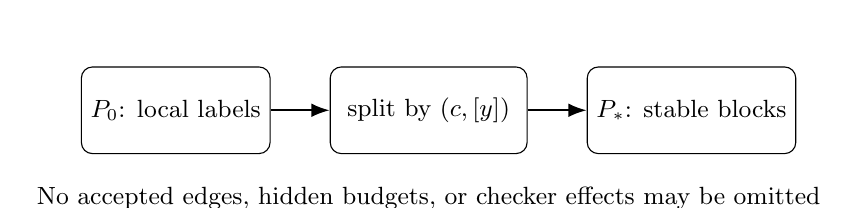
\begin{tikzpicture}[>=Latex, every node/.style={font=\small},node distance=0.45cm]
\node[draw,rounded corners,minimum width=2.25cm,minimum height=1.1cm] (a) {$P_0$: local labels};
\node[draw,rounded corners,right=0.75cm of a,minimum width=2.5cm,minimum height=1.1cm] (b) {split by $(c,[y])$};
\node[draw,rounded corners,right=0.75cm of b,minimum width=2.5cm,minimum height=1.1cm] (c) {$P_*$: stable blocks};
\draw[->,thick](a)--(b);\draw[->,thick](b)--(c);
\node[below=0.3cm of b,align=center] {No accepted edges, hidden budgets, or checker effects may be omitted};
\end{tikzpicture}
\caption{The finite search is over partitions of the supplied transition graph, not all possible machines.}
\end{figure}

\begin{theorem}[Finite constructive future quotient]\label{thm:refine}\hypertarget{stmt:refine}{}
For a finite contract-labeled game with $n=|X|$, the refinement procedure reaches a stable partition $P_*$ after at most $n-|P_0|$ strict splitting rounds. Its equivalence $\sim_*$ is the coarsest stable equivalence that respects $\ell$: every other equivalence respecting labels and matching costed successor classes refines $P_*$. The partition is effectively computable from the explicit graph.
\end{theorem}\backproof{refine}

The coarseness assertion concerns \emph{the chosen strong local matching criterion}. It does not assert that this quotient has the fewest states among every conceivable abstraction preserving only one numerical value. Strong equivalence can retain information that a single fixed target does not need.

\begin{corollary}[Finite exact preservation of forcing]\label{cor:val}\hypertarget{stmt:val}{}
Let $T$ be the target set encoded in the label. Every $x$ satisfies
\[
 V_G(x)=V_{G/\sim_*}([x]_{P_*}).
\]
This remains true for every nonnegative integer budget threshold and for the existence of a force-reaching controller strategy, provided all admitted edges and their costs are explicitly represented.
\end{corollary}\backproof{val}

\section{A replayable quotient certificate}
\begin{definition}[Finite partition certificate]
The proposed quotient certificate contains: (i) the frozen graph's version/hash and complete vertex, edge, cost, and label table; (ii) a block identifier $q(x)$ for each state; (iii) for each block, the common label and common set of pairs $(c,q(y))$; and (iv) a declaration of which target and cost queries are being preserved. A checker recomputes every signature from the frozen graph and accepts only if the common-label and common-successor conditions hold.
\end{definition}

\begin{proposition}[A local witness suffices for an exact global planning claim]\label{prop:check}\hypertarget{stmt:check}{}
If a finite partition certificate passes the described deterministic checker, the represented quotient preserves the exact forced value of every vertex. The certificate does not need to contain or trust a table of those values.
\end{proposition}\backproof{check}

This is useful because a small local condition can certify a global infinite-play statement \emph{relative to the fully specified finite graph}. The checker does not validate that the graph itself represents the true deployed machine, that all physical costs are correctly measured, or that a discovered partition is the coarsest unless the refinement proof or algorithm is separately supplied.

\begin{figure}[ht]
\centering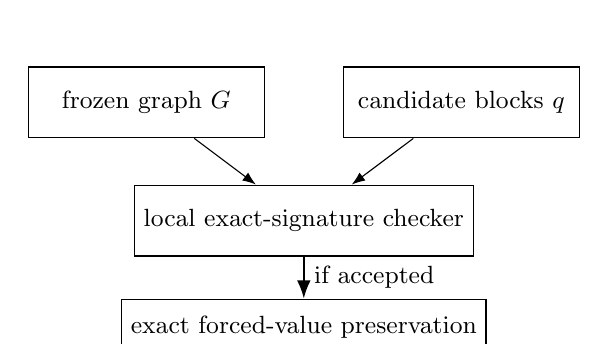
\begin{tikzpicture}[>=Latex,every node/.style={font=\small}]
\node[draw,minimum width=3cm,minimum height=.9cm] (g) at (0,0) {frozen graph $G$};
\node[draw,minimum width=3cm,minimum height=.9cm] (q) at (4,0) {candidate blocks $q$};
\node[draw,minimum width=4cm,minimum height=.9cm] (v) at (2,-1.5) {local exact-signature checker};
\draw[->](g)--(v);\draw[->](q)--(v);
\node[draw,minimum width=4cm,minimum height=.7cm] (r) at (2,-2.85) {exact forced-value preservation};
\draw[->,thick](v)--node[right]{if accepted}(r);
\end{tikzpicture}
\caption{A small replayable check discharges a mathematical quotient obligation, not deployment fidelity.}
\end{figure}

\section{Why attractive weaker summaries are unsound}
\begin{example}[Retrospective equivalence loses a winning strategy]\label{ex:retro}
Take two controller states $x,x'$ with the same current report ``no accepted target yet''. From $x$ there is a cost-one transition to the target $t$; from $x'$ there is only a cost-zero self-loop. The retrospective report $Q(x)=Q(x')$ is preserved by merging the two states, yet the true forced values are $1$ and $+\infty$. A quotient that exports either one as the common value is incorrect. The hidden fact is which future edges are legal.
\end{example}

\begin{example}[Equal values need not imply future equivalence]\label{ex:eqcost}
Let $x\to t$ cost $1$, let $z\to t$ cost $0$, and let $y\to z$ cost $1$, where $t$ is the only target. All nonterminal states are controller-owned. Then $V(x)=V(y)=1$, but $x$ has a cost-one edge directly to a target block while $y$ has a cost-one edge to a nonterminal block. A value-only partition merges $x$ and $y$; the local stable partition separates them. Thus a value-equal compression can be adequate for one retrospective numerical query yet inadequate for updating policies or changing the target.
\end{example}

\begin{figure}[ht]
\centering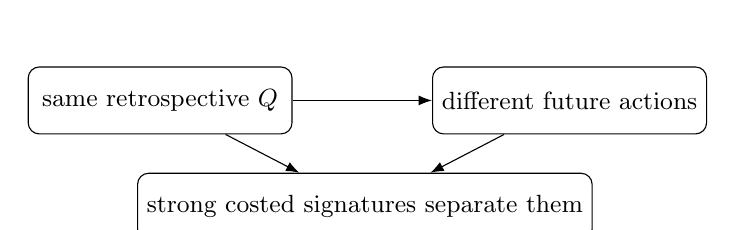
\begin{tikzpicture}[>=Latex,every node/.style={font=\small}]
\node[draw,rounded corners,minimum width=3.35cm,minimum height=.85cm] (a) at (0,0) {same retrospective $Q$};
\node[draw,rounded corners,minimum width=3.35cm,minimum height=.85cm] (b) at (5.2,0) {different future actions};
\node[draw,rounded corners,minimum width=4cm,minimum height=.85cm] (c) at (2.6,-1.35) {strong costed signatures separate them};
\draw[->](a)--(b);\draw[->](a)--(c);\draw[->](b)--(c);
\end{tikzpicture}
\caption{Retrospective equality is weaker than future decision sufficiency.}
\end{figure}

\begin{proposition}[Changing the contract can invalidate a proven quotient]\label{prop:newcontract}\hypertarget{stmt:newcontract}{}
A partition stable for a contract $K$ need not be stable after changing the required target observation, transition costs, checker requirements, or permitted actions. A new contract version therefore requires a fresh stability check unless the earlier certificate already explicitly covers the changed quantities.
\end{proposition}\backproof{newcontract}

\section{The economic cost of computing a faithful quotient}
Let $p$ be the fully charged per-episode planning and execution cost before compression and $q$ after compression, for a frozen common workload, and let $B$ include \emph{all} quotient construction, validation, migration, retained ledger, and failed search charges. For $N$ episodes, strict net benefit follows from $N(p-q)>B$ if $p>q$ and the admitted outcomes remain equivalent. The quotient theorem establishes outcome preservation; it does not establish $p>q$. A quotient with a million-state checker may be mathematically exact and economically unprofitable.

\begin{theorem}[Conditional payoff of a certified planning quotient]\label{thm:payoff}\hypertarget{stmt:payoff}{}
Suppose a local partition certificate establishes exact forced-cost equivalence between a finite model and its quotient. Suppose further that an externally stipulated fully charged comparison under the \emph{same} contract proves per-episode bounds $C_{\rm old}\ge p$ and $C_{\rm new}\le q$, with $p>q$, and aggregate additional charges at most $B$. Then $N(p-q)>B$ certifies strictly lower total cost for $N$ required episodes against the declared old policy, while preserving the represented target-forcing guarantee.
\end{theorem}\backproof{payoff}

The two parts of the conclusion have different certificates. Signatures certify \emph{planning semantics}; cost inequalities certify \emph{economic advantage}. Neither alone entails the other. The stronger claim that no equally informed alternative machine performs better remains unsupported without exhaustive or otherwise valid competitor reasoning.

\section{Limits, alternatives, and the next question}
A complete finite graph permits an exact quotient. But an effective theorem prover can encounter certificates of unknown future availability, hidden scheduler actions, unbounded history, or fresh obligations that make a finite exact state summary unavailable or prohibitively expensive. A machine might know the current architecture while not knowing which receipt will be accepted tomorrow.

In particular, two states with different hidden evidence may have the same public observation but different safe actions. This is not a defect of stable-partition mathematics; it is a limitation on the \emph{controller's information}. W3 therefore changes the main question from ``which states are behaviorally identical?'' to ``how much information must the controller actually receive to force a certified target?''

\section{Research, comparison, and verification ledger}
\small
\begin{longtable}{p{0.17\linewidth}p{0.38\linewidth}p{0.33\linewidth}}
\toprule Status & Mathematical contribution & Basis and limitation \\\midrule\endhead
Inherited & Retrospective observational sufficiency & W0 V.4: factorization of required observations \\
Inherited & Forced cost for explicit finite games & W0 VI.5; W1 exact quotient preservation \\
Derived / candidate-original relative to W0--W1 & Theorem~\ref{thm:refine}: coarsest stable contract-labeled partition from finite refinement & Constructive proof below; no broad literature originality claim \\
Derived & Corollary~\ref{cor:val}, local certificate proposition & Depends on W1 strong quotient theorem \\
Counterexample & Equal current reports and equal forced values insufficient for strong planning equivalence & Explicit finite graphs in Section 5 \\
Conditional & Quotient economic payoff & Requires independently justified comparison bounds in addition to quotient semantics \\
Unresolved & Exact finite abstraction of an unrestricted evolving theorem prover & May be undecidable or depend on unbounded history \\
\bottomrule
\end{longtable}
\normalsize


\section{Competing Level-2 research directions}
Two mathematical departures from W1 were compared. The first sought an efficient quotient construction that is certified without first computing all game values; it led to local costed-successor signatures and finite partition refinement. The second sought minimal retrospective score summaries; it can merge more states for a fixed observation, but the counterexamples above show that such a summary cannot generally be used to synthesize future safe actions. The final work keeps the first as its central theorem and retains the second as a precise limitation. Neither approach implies a general-purpose semantic-equivalence algorithm for arbitrary programs.

An Atlas-style internal audit checked the inductive refinement invariant, zero-cost cycles, the distinction between strong bisimulation and value equality, the frozen checker labels, and cost claims. The most important restriction is that the algorithm is \emph{constructive on an already finite graph}, not a proof that an evolving ATP's infinite history has a sufficient finite quotient. The larger manuscript W0, and W1, are retained unchanged as independent prior stages.

\section{PROOFS}
\hypertarget{proof:refine}{}\subsection*{Theorem \ref{thm:refine}: finite refinement} \backstatement{refine}
Each splitting step refines its predecessor; it never merges distinct blocks. Every strict split increases the number of nonempty blocks by at least one, and the number never exceeds $n$. Therefore there are at most $n-|P_0|$ strict rounds. Once a round makes no split, each block has a single label and common successor signature, hence is stable; repeating the calculation changes nothing.

Let $R$ be any stable equivalence respecting labels. Initially each $R$-class lies in one $P_0$ block. Suppose it lies in one $P_k$ block. Two $R$-equivalent states have matching costed successor $R$-classes by $R$-stability. Since each $R$-class lies within one $P_k$ block, replacing $R$-class identifiers by the containing $P_k$-block identifiers yields equal $S_{P_k}$ signatures. They cannot be separated in $P_{k+1}$. By induction, every $R$-class is contained in a final block of $P_*$. Thus $P_*$ is coarsest among stable label-respecting equivalences. All operations are finite enumeration, label comparison, and set equality on the supplied graph.

\hypertarget{proof:val}{}\subsection*{Corollary \ref{cor:val}: forcing preservation} \backstatement{val}
Stability says exactly that the final equivalence has matching ownership, target status, and costed successor classes. Hence it is an exact costed game congruence in W1's sense. Apply W1's quotient theorem, whose budget-expanded attractor proof treats zero-cost loops as possible infinite avoidance and consequently preserves finite forced values and $+\infty$.

\hypertarget{proof:check}{}\subsection*{Proposition \ref{prop:check}: local checker} \backstatement{check}
The checker exhaustively compares the input graph's labels and the cost/block pairs of every state with those claimed for its block. Acceptance implies stability by definition. The preceding corollary supplies the global consequence. The output of any separately supplied numeric solver is irrelevant to this inference.

\hypertarget{proof:newcontract}{}\subsection*{Proposition \ref{prop:newcontract}: changed contracts} \backstatement{newcontract}
As a witness, merge two states with identical old labels and identical transitions, then change the target flag of one but not the other. The old partition was stable, while the required common-label condition now fails. Alternatively, change one edge cost while retaining destinations: the common successor signatures may differ. These are explicit counterexamples to automatic stability under a changed contract.

\hypertarget{proof:payoff}{}\subsection*{Theorem \ref{thm:payoff}: economic condition} \backstatement{payoff}
Exact target-forcing semantics follow from the accepted quotient certificate and Corollary~\ref{cor:val}. For economic charges, the old policy consumes at least $Np$ over the frozen episodes. The quotient policy consumes no more than $Nq+B$. Strict inequality $N(p-q)>B$ is equivalent to $Nq+B<Np$. These two independently established statements yield the conjunction, with no implication of universal optimality or physical measurement.
\section*{Source and verification notes}
\addcontentsline{toc}{section}{Source and verification notes}
The sole mathematical research input for this development was the user-supplied 68-page manuscript \emph{Certified Self-Improving Mathematical Discovery: Parts II--VI}, strengthened ATLAS v2 edition dated 15 November 2026 (here called W0). Section references to W0 are internal source attributions, not claims that its original external bibliography has been independently consulted. W0 itself identifies ChatGPT (OpenAI) as its editorial author and Brian Tenneson as research director. W0 remains unaltered. The new research articles are AI-assisted drafts under Brian Tenneson's research direction; their mathematical novelty has only been compared with the supplied ancestry, not with the wider literature.

All proofs in this manuscript are human-readable paper arguments, reviewed internally but \emph{not} independently formally checked. Any finite checker mentioned is part of the stated mathematical model. No deployed FORGE-6/CAMI machine, hardware benchmark, new experiment, or independent proof-kernel receipt is represented as having occurred. Claims about external priority, unrestricted computation, and improvement of any real implementation remain open.

\section*{AI disclaimer and attribution}\addcontentsline{toc}{section}{AI disclaimer and attribution}
This research exposition and its diagrams were drafted with AI assistance, with research direction attributed to Brian Tenneson. AI assistance does not substitute for independent proof checking or external mathematical peer review. Historical authorship of W0 is preserved in the source and verification notes. The conditional theorems here concern explicit mathematical contracts, not autonomous self-modification of ChatGPT or proof of machine consciousness.

\section*{Independent-review boundary}\addcontentsline{toc}{section}{Independent-review boundary}
For W2, an external reproducer would need the exact finite state graph, the contract labels, a complete list of charged successors, and the partition map. The local checker can test the partition certificate without trusting a claimed optimal-cost table. The following diagram isolates the evidence transitions that have and have not been performed.
\begin{figure}[ht]\centering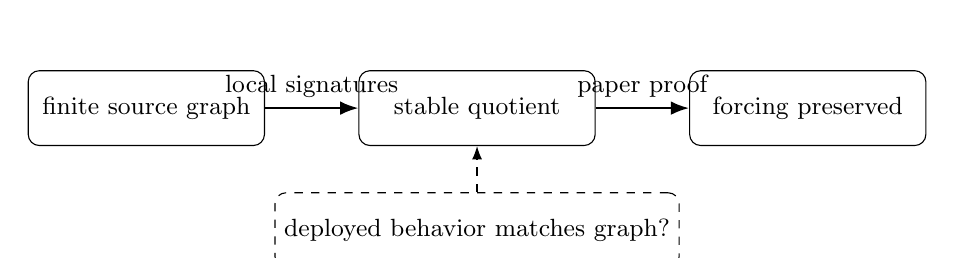
\begin{tikzpicture}[>=Latex,every node/.style={font=\small}]
\node[draw,rounded corners,minimum width=3cm,minimum height=.95cm] (a) at (0,0) {finite source graph};
\node[draw,rounded corners,minimum width=3cm,minimum height=.95cm] (b) at (4.2,0) {stable quotient};
\node[draw,rounded corners,minimum width=3cm,minimum height=.95cm] (c) at (8.4,0) {forcing preserved};
\draw[->,thick](a)--node[above]{local signatures}(b);
\draw[->,thick](b)--node[above]{paper proof}(c);
\node[draw,dashed,rounded corners,minimum width=4cm,minimum height=.95cm] (d) at (4.2,-1.55) {deployed behavior matches graph?};
\draw[dashed,->](d)--(b);
\end{tikzpicture}\caption{Finite graph certification does not certify the unverified deployed-model correspondence.}\end{figure}
The source manuscript, earlier completion, original assumptions, and all rejected or unresolved obligations remain separate historical artifacts; a stable partition is a compressed controller representation, not a license to discard them.

\end{document}
